\section{Results and discussion}\label{sec:results}
\subsection{Reference solution and seven-case comparison}
% R1: reference profiles
The refined Case 3C solution links \COtwo{} uptake to the predicted fugacity, speciation and temperature profiles (\cref{fig:reactive-case3c-profiles}).
It predicts \qty{91.55}{\percent} capture against \qty{89.50}{\percent} observed, with peak liquid temperature \qty{347.86}{K} (\cref{tab:reactive-numerical-verification} gives full precision).
The vapor-to-liquid \COtwo{} fugacity difference remains positive but narrows through most of the bed as cumulative capture flattens.
Toward the lean inlet, free MEA increases while protonated MEA and carbamate decrease, showing the changing bulk composition supplied to the film calculation.
These profiles show the bulk quantities supplied to the film approximation; they are not independent measurements of speciation.


\begin{figure}[pos=htbp]
\centering
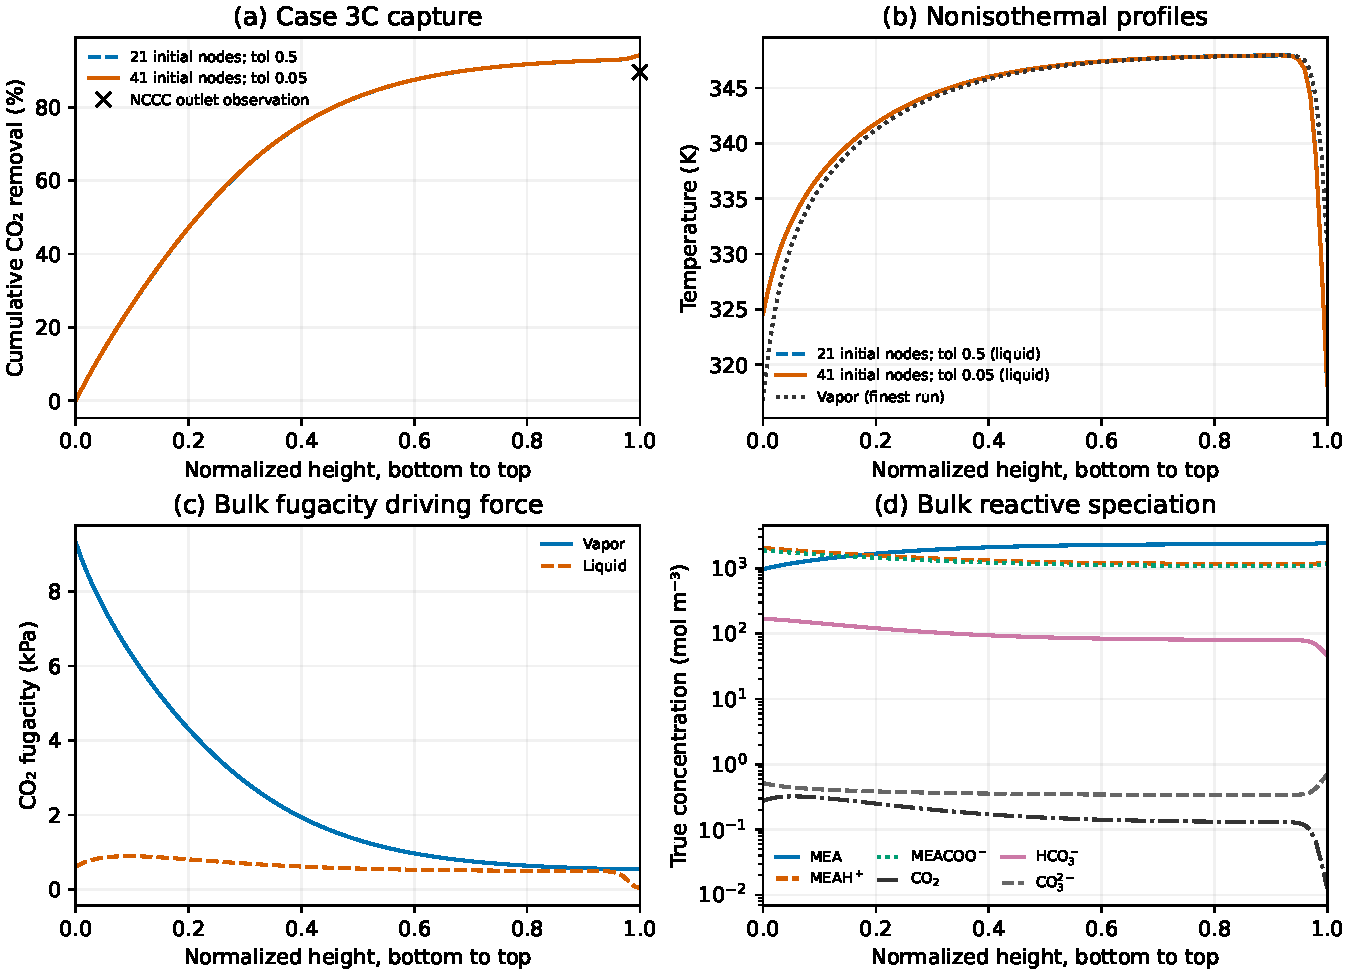
\includegraphics[width=0.98\textwidth]{figures/reactive-case3c-profiles.pdf}
\caption{Coupled nine-species Case 3C profiles with conventional reaction enhancement. The 21- and 41-point initial meshes use collocation tolerances of 0.5 and 0.05. The cross in panel (a) is reported outlet capture (Morgan et al.\ \cite{Morgan2020}); curves are calculated profiles. Panels (c) and (d) use the refined calculation, and panel (d) shows six principal species from the nine-species equilibrium solution. Capture is in percent, temperature in kelvin, fugacity in kilopascals and concentration in \unit{mol.m^{-3}}. Normalized position runs from vapor inlet at 0 to liquid inlet at 1.}
\label{fig:reactive-case3c-profiles}
\end{figure}


\subsubsection*{Numerical verification and computational cost}
% R2: observed refinement
The joint mesh/tolerance refinement changes Case 3C capture by \num{0.005} percentage points and peak liquid temperature by \qty{0.045}{K} (\cref{tab:reactive-numerical-verification}).
Both calculations take two mesh iterations and add one node; the maximum normalized RMS residual decreases from \num{0.125340} to \num{0.043138}, with zero maximum scaled boundary residual.
All nine species remain positive, and net \COtwo{} and water flows vary by less than \qty{3e-14}{mol.s^{-1}} over the exported positions.
At 10,001 sampled positions, the finest additional Case 3C refinement (81 to 121 nodes, tolerance \num{5e-5}) gives an axial net-enthalpy-flow range of \qty{0.134}{W}; its capture differs from the paired refined calculation by less than \num{0.0001} percentage points (\cref{tab:run-diagnostics}).

\begin{table}[pos=htbp]
  \centering
  \caption{Observed joint mesh/tolerance refinement response for the coupled nine-species Case 3C calculation. Both calculations use the same equations and parameters. The iteration rows show the printed maximum normalized RMS residual after each mesh iteration; final residuals below retain additional precision.}
  \label{tab:reactive-numerical-verification}
  \small
  \renewcommand{\arraystretch}{1.12}
  \begin{tabularx}{\textwidth}{@{}Xrr@{}}
    \toprule
    Quantity & Coarser calculation & Refined calculation \\
    \midrule
    Initial / final mesh nodes & 21 / 22 & 41 / 42 \\
    Collocation tolerance & 0.5 & 0.05 \\
    Mesh iterations & 2 & 2 \\
    Maximum RMS residual, iterations 1 $\to$ 2 & $1.64\to0.123$ & $0.0507\to0.0393$ \\
    Final maximum RMS residual & 0.122785 & 0.039322 \\
    Maximum scaled boundary residual & 0 & 0 \\
    Column RHS evaluation batches & 27 & 17 \\
    Jacobian evaluation batches & 6 & 4 \\
    State Jacobian evaluations & 125 & 164 \\
    Liquid equilibrium solves, including profile output & 608 & 551 \\
    \COtwo{} capture (\unit{\percent}) & 94.19959 & 94.20397 \\
    Peak liquid temperature (\unit{K}) & 347.9682 & 347.9399 \\
    Net-enthalpy-flow range, 101 positions (\unit{W}) & 286.440 & 267.572 \\
    \bottomrule
  \end{tabularx}
  \par\smallskip
  \begin{minipage}{\textwidth}\footnotesize
    The continuous equations predict zero net-enthalpy-flow range; the nonzero numerical values are diagnostics, with no asserted energy-error threshold. RHS denotes the right-hand side of the column equations. A batch evaluates all nodes or interval midpoints, not a single axial state. Four Jacobian batches correspond to two node/midpoint pairs. Mesh iterations count outer refinement cycles, not inner Newton steps. Both calculations use boundary tolerance \num{0.001} and a 1000-node limit. Peak memory is reported with the timing study.
  \end{minipage}
\end{table}


% R3: separately measured cost
The three coarse Case 3C repeats have a median BVP wall time of \qty{34.66}{s}, spanning \qtyrange{34.41}{34.89}{s}.
The fastest run uses \qty{34.23}{s} process CPU time and \qty{51.45}{s} total wall time, with peak resident memory \num{203.51} MiB, 21 initial and 22 final nodes, and two mesh iterations.

\subsubsection*{Seven-case comparison}
% R4: capture agreement
Capture agreement varies substantially across the seven NCCC cases (\cref{fig:reactive-seven-case-capture}).
The equally weighted mean absolute error is \num{5.85} percentage points, with the largest signed errors of \num{+11.45} points for Case 6C and \num{-11.93} points for Case 7C.
The opposite signs show that the model does not have a uniform capture bias over these conditions.


\begin{figure}[pos=htbp]
\centering
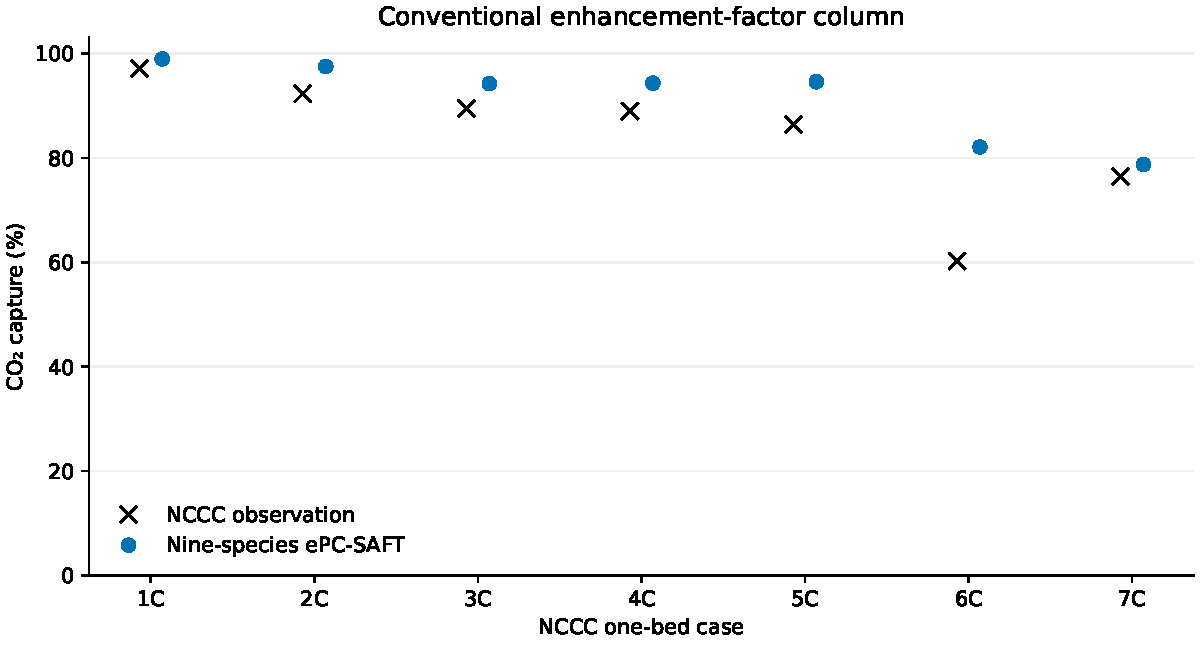
\includegraphics[width=0.9\textwidth]{figures/reactive-seven-case-capture.pdf}
\caption{Predicted and reported capture for NCCC Cases 1C--7C using the coupled nine-species model and observations from Morgan et al.\ \cite{Morgan2020}. Signed errors are prediction minus observation, in percentage points; mean absolute error is \num{5.85} percentage points.}
\label{fig:reactive-seven-case-capture}
\end{figure}


% R5: specific thermal observations
The packing-temperature comparisons expose differences in predicted temperature level and axial shape (\cref{fig:generated-temperature-profiles}).
For Case 3C, both phase curves approach the upper-bed taps near $\zeta=0.6$ and 0.8, but lie above the tap near $\zeta=0.2$; its coarse calculation has \qty{91.54}{\percent} capture and peak liquid temperature \qty{347.91}{K}.
Case 4C overpredicts the three upper taps, while Case 7C predicts a broad elevated-temperature region that is absent from the reported profile, particularly near $\zeta=0.8$.


\begin{figure}[pos=htbp]
\centering
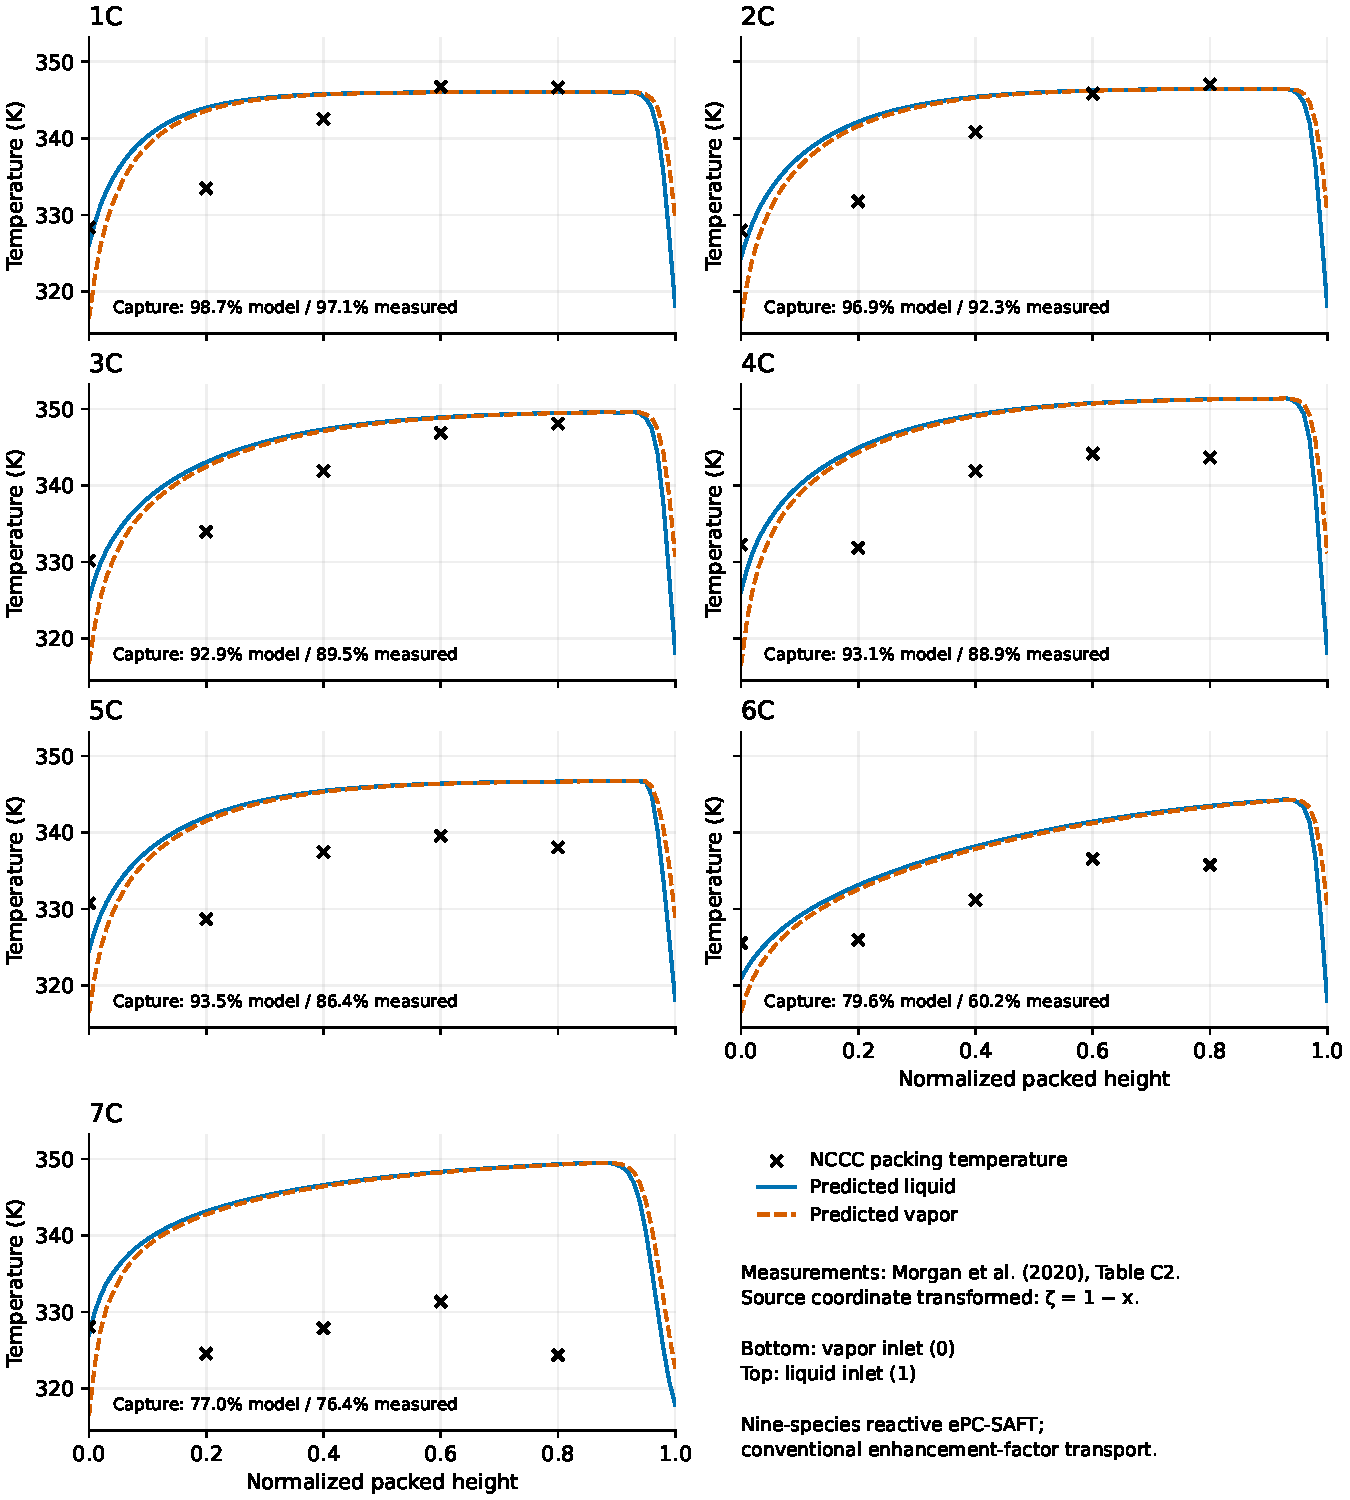
\includegraphics[width=0.98\textwidth]{figures/reactive-seven-case-temperatures.pdf}
\caption{Temperature profiles for the seven one-bed NCCC 2017 C cases. Solid and dashed curves denote liquid and vapor temperatures calculated with coupled nine-species reactive ePC-SAFT and conventional reaction enhancement. Crosses are reported packing temperatures from Table C2 of Morgan et al.\ \cite{Morgan2020}, converted to kelvin and normalized bottom-to-top height $\zeta=1-x$, where $x$ is the source coordinate. The vapor inlet is at zero and liquid inlet at one. The source does not specify a phase-specific sensor designation. Cases 1C--3C use the \qty{318.15}{K} lean-inlet assumption in \cref{tab:nccc-one-bed-scope}.}
\label{fig:generated-temperature-profiles}
\end{figure}


% R6: campaign numerical scope
All seven calculations converge at the campaign settings (\cref{tab:run-diagnostics}), while physical agreement remains uneven. Only Case 3C has the paired refinement, which provides a comparison magnitude for the perturbation responses that follow.
\FloatBarrier

\subsection{Thermodynamic and transport sensitivity}
% R7: thermodynamic capture response
Among the tested equal relative thermodynamic changes, the MEA--water interaction produces the largest capture response (\cref{fig:reactive-parameter-sensitivity}).
Its 0.95 and 1.05 multipliers change capture by \num{-0.82} and \num{+0.76} percentage points from the refined \qty{91.55}{\percent} baseline.
The remaining response magnitudes decrease in the order R5, R4 and \COtwo--water: their paired capture changes are \num{+0.59}/\num{-0.60}, \num{+0.42}/\num{-0.42} and \num{+0.16}/\num{-0.17} points.
Every capture change exceeds the \num{0.005}-point reference refinement difference, but the perturbed range of \qtyrange{90.73}{92.31}{\percent} still exceeds the observed \qty{89.50}{\percent}.


\begin{figure}[pos=htbp]
\centering
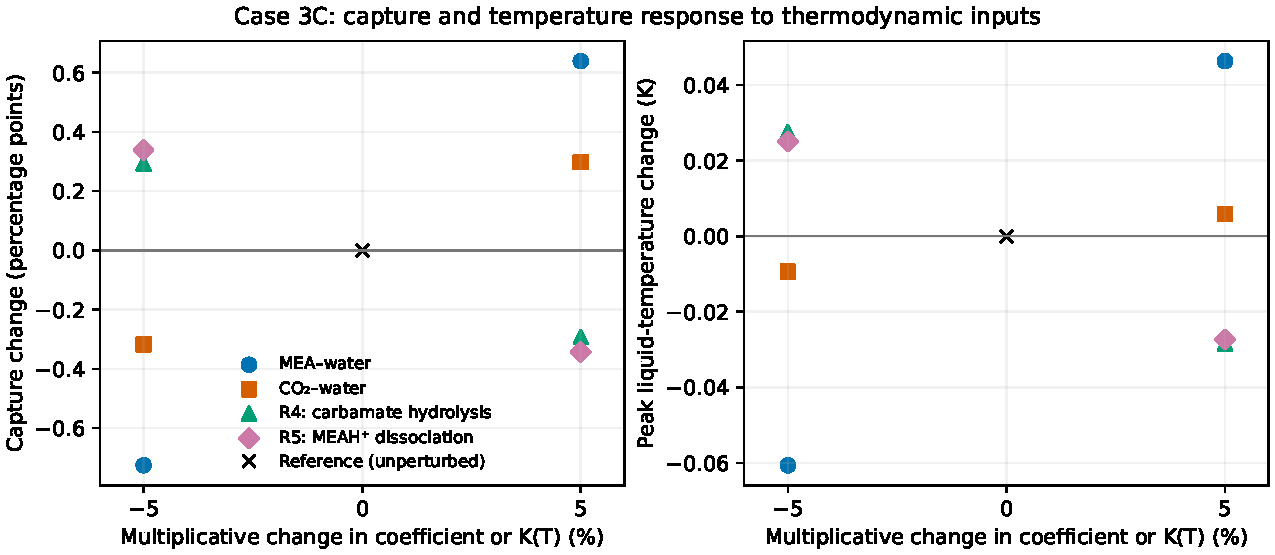
\includegraphics[width=0.98\textwidth]{figures/reactive-parameter-sensitivity.pdf}
\caption{Thermodynamic sensitivity of the coupled nine-species Case 3C model. Points represent separate calculations with one binary interaction coefficient or equilibrium constant multiplied by 0.95 or 1.05; crosses denote the unperturbed reference. R4 denotes carbamate hydrolysis and R5 protonated-MEA dissociation. The reference uses 41 initial nodes and tolerance 0.05, with capture \qty{91.54839}{\percent} and peak liquid temperature \qty{347.86155}{K}. Capture changes are in percentage points and peak liquid-temperature changes are in kelvin.}
\label{fig:reactive-parameter-sensitivity}
\end{figure}


% R8: thermodynamic temperature response
The corresponding peak-temperature changes are small and only partly exceed the \qty{0.045}{K} refinement difference.
MEA--water gives \qty{-0.11}{K} and \qty{+0.10}{K}.
The corresponding R4 changes are \qty{+0.06}{K} and \qty{-0.06}{K}, R5 changes are \qty{+0.06}{K} and \qty{-0.07}{K}, and \COtwo--water changes are \qty{+0.016}{K} and \qty{-0.017}{K}.
The reaction-constant effects modestly exceed it, while the \COtwo--water effects fall below it.

% R9: transport capture response
The liquid-side transfer coefficient has the largest capture effect among the three tested transport inputs (\cref{fig:transport-sensitivity}).
Multipliers of 0.9 and 1.1 give capture changes of \num{-0.53}/\num{+0.40} percentage points, compared with \num{+0.28}/\num{-0.29} for viscosity and \num{+0.08}/\num{-0.09} for free molecular \COtwo{} diffusivity.
The factor-one control reproduces the reference.
All six responses exceed the reference capture refinement difference.


\begin{figure}[pos=htbp]
\centering
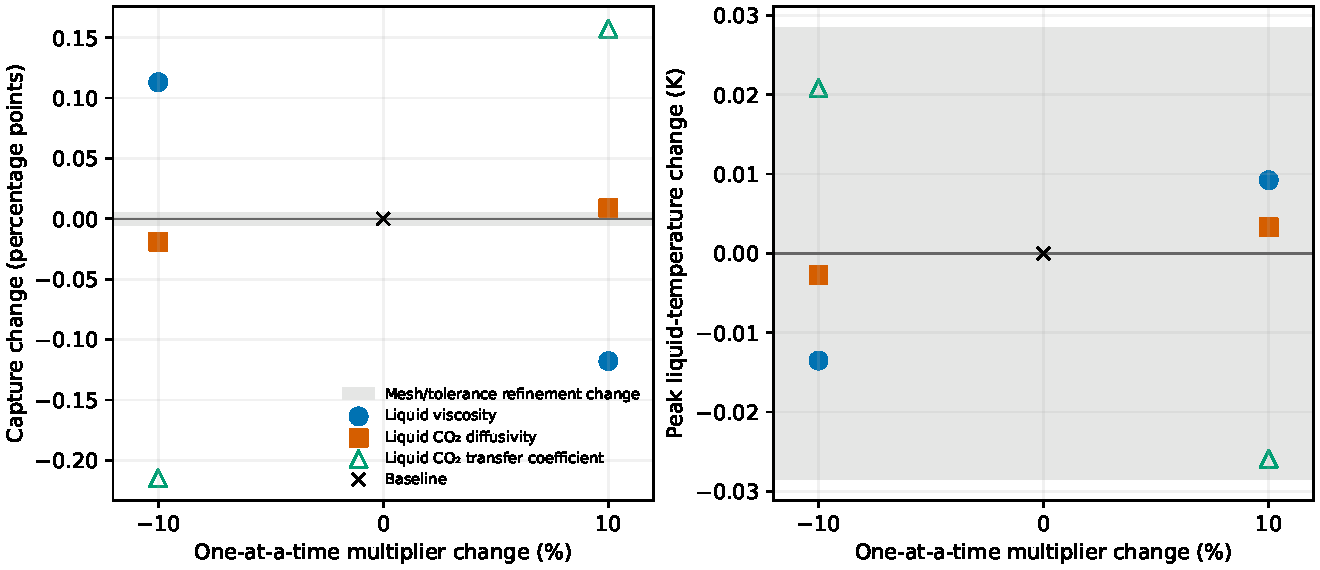
\includegraphics[width=0.98\textwidth]{figures/transport-sensitivity.pdf}
\caption{Transport sensitivity of the coupled nine-species Case 3C model. Points denote separate calculations with liquid viscosity, free liquid \COtwo{} diffusivity or the liquid-side \COtwo{} transfer coefficient multiplied by 0.9 or 1.1, including recalculation of dependent transport and enhancement quantities. The cross denotes the refined reference, with capture \qty{91.54839}{\percent}; capture changes are in percentage points and peak liquid-temperature changes in kelvin. Shading shows the magnitude of the joint mesh/tolerance refinement change.}
\label{fig:transport-sensitivity}
\end{figure}


% R10: coupled transport interpretation
The negative capture response to increased molecular \COtwo{} diffusivity is consistent with the recalculated enhancement and transfer resistances.
For the 1.1 multiplier, median perturbed/reference ratios at matched axial positions are \num{1.047} for $k_L$, \num{0.931} for enhancement and \num{0.975} for their product.
These ratios compare separately solved profiles at matched axial positions.
All peak-temperature changes are below \qty{0.037}{K}, smaller than the \qty{0.045}{K} refinement difference; their signs and ordering are not resolved by that comparison.

% R10b: actual applicability
The baseline calculation extends beyond the documented source ranges of two adopted transport descriptions (\cref{tab:transport-applicability}).
Its Hatta numbers of approximately 320--698 exceed the enhancement source comparison range of 35--165 throughout the profile.
Its peak temperature of \qty{347.86}{K} also exceeds the MEA diffusivity source's \qty{333}{K} upper temperature; the other diffusivity correlations have no documented upper temperature limit.
\FloatBarrier

\subsection{Operating response}\label{sec:operating-response}
% R11: discrete operating results
Six of the seven operating conditions converged, including the coarse baseline with \qty{91.54}{\percent} capture (\cref{fig:operating-response}).
Increasing liquid flow by ten percent at fixed reported dry-gas flow raises capture by \num{0.31} percentage points.
Lean loadings 0.225 and 0.275 mol \COtwo{} per mol MEA give changes of \num{+3.75} and \num{-6.86} points relative to 0.25, while liquid-inlet temperatures \qty{313.15}{K} and \qty{323.15}{K} give \num{+0.11} and \num{-0.08} points relative to \qty{318.15}{K}.


\begin{figure}[pos=htbp]
\centering
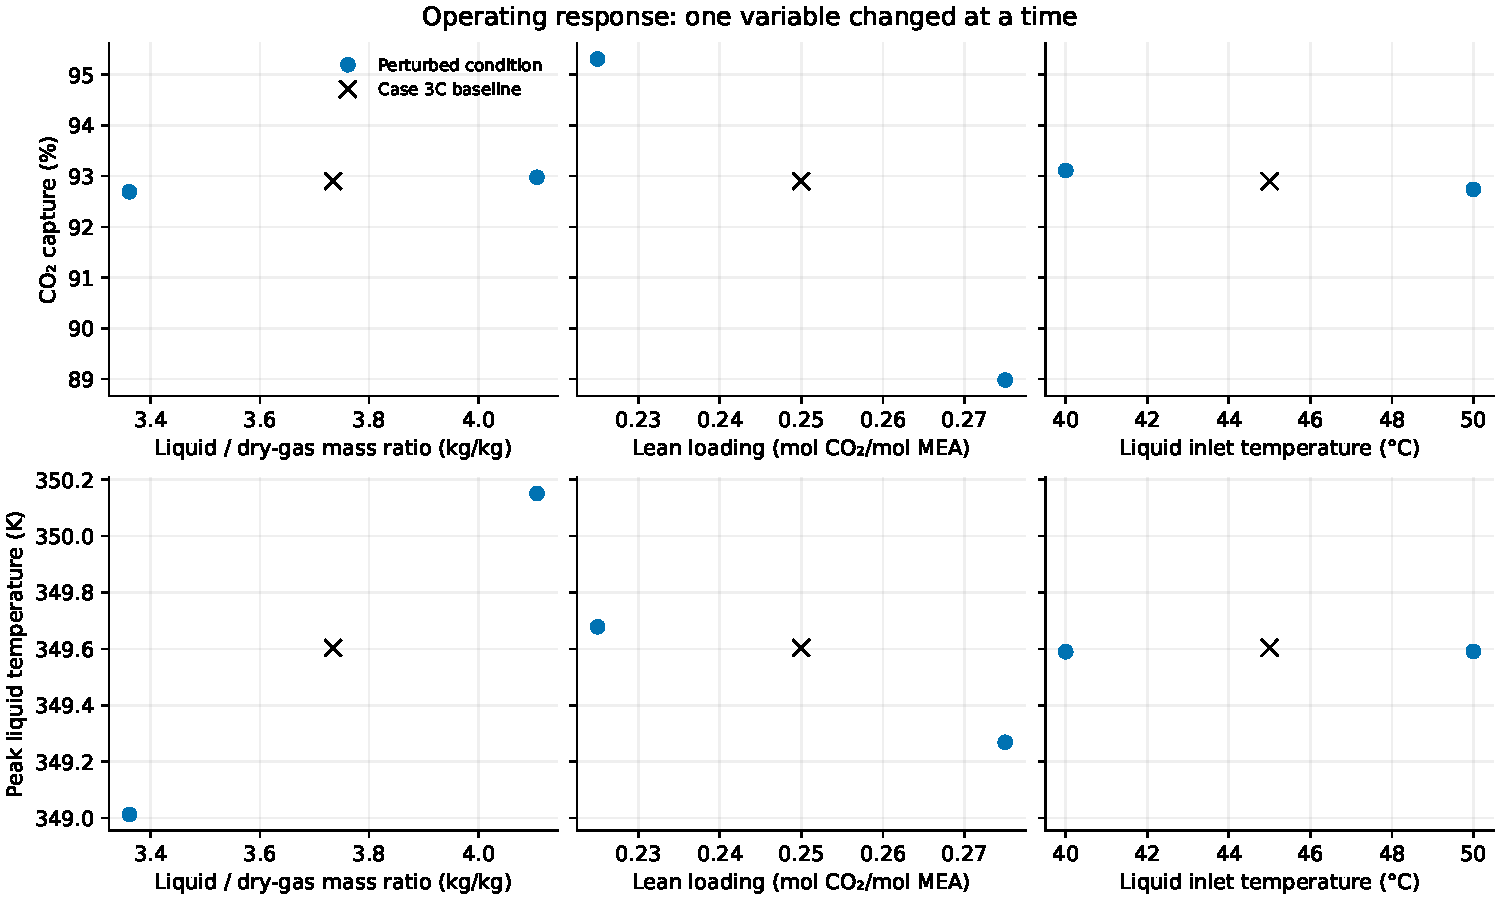
\includegraphics[width=0.98\textwidth]{figures/reactive-operating-response.pdf}
\caption{Operating response of the coupled nine-species Case 3C model. Circles denote discrete one-at-a-time predictions; crosses denote the unperturbed baseline. The baseline has $L/G=3.73423$ (liquid mass/reported dry gas mass), loading 0.25 mol \COtwo{} per mol MEA and liquid-inlet temperature \qty{318.15}{K}. Capture is in percent and peak liquid temperature in kelvin. Liquid mass flow changes at fixed reported dry-gas flow for the mass-ratio comparison. The lower liquid-to-gas condition did not converge and is omitted.}
\label{fig:operating-response}
\end{figure}


% R12: joint capture and temperature interpretation
Lower lean loading increases available solvent capacity and gives the largest positive capture response among these specified changes.
Lower loading raises free MEA and lowers the liquid \COtwo{} fugacity; near the gas inlet, this increases the modeled driving force.
Peak liquid-temperature changes are \qty{+0.61}{K} for higher liquid flow and \qty{+0.25}{K}/\qty{-0.83}{K} for the two loading changes.
The colder and warmer liquid inlets give peak changes of \qty{+0.02}{K} and \qty{-0.01}{K}, both below the refinement difference.

\FloatBarrier

\subsection{Interpretation and future work}
% R14: integrated interpretation
The calculations connect reactive bulk thermodynamics to column response, while physical disagreement persists despite small capture changes under the tested refinement.
The refined Case 3C capture error of \num{2.05} percentage points is much larger than its \num{0.005}-point refinement change, and Cases 6C and 7C have still larger physical discrepancies.
The reduced vapor-EOS composition and the extrapolated enhancement and transport correlations limit interpretation; their individual contributions to the error are not resolved.
The lean-inlet temperature assumed for Cases 1C--3C is a bounded input uncertainty: in Case 3C, liquid-inlet temperatures of \qty{313.15}{K} and \qty{323.15}{K} change capture by \num{+0.11} and \num{-0.08} percentage points relative to \qty{318.15}{K} (\cref{sec:operating-response}), small against the \num{2.05}-point refined capture error.

% R15: limitations and next steps
The film, parameter and optimization questions raised by these results were examined with a twelve-state conserved formulation of the same absorber, discretized in conservative upwind cells and solved with IPOPT \cite{Wachter2006}.
This formulation differs from the nine-species model reported above, so its capture errors are not directly comparable with the \num{5.85}-point mean absolute error of that model.
A finite-rate reactive film computes \COtwo{} transfer from ePC-SAFT bulk and interfacial speciation, with an \NtwoO{}-analogy Henry constant and no empirical enhancement factor.
Across Cases 2C--7C at 129 axial nodes, its capture mean absolute error is \num{5.45} percentage points, against \num{6.05} for an equilibrium-manifold film and \num{6.28} for the enhancement factor; this order holds at 17, 33, 65 and 129 nodes, and Case 1C is omitted because the enhancement-factor calculation did not converge on the two finest meshes.
Mesh refinement raises the error of all three films, and at 129 nodes all three underpredict Case 7C capture by \num{8.8} to \num{17.4} percentage points, with changes of \num{1.6} to \num{1.8} points still occurring between 65 and 129 nodes, so Case 7C is not resolved with respect to the axial mesh.
With the jointly fitted MEA parameter set, which also changes the reaction and caloric inputs, the seven-case capture mean absolute error at 33 nodes is \num{4.58} percentage points, against \num{4.79} with the earlier set; without Case 7C, the earlier set is better at \num{4.27} against \num{4.87} points, so the joint fit does not consistently improve the absorber prediction.
Constrained optimization with exact first derivatives was verified for the minimum solvent flow that gives \qty{90}{\percent} capture in Case 3C with the equilibrium-manifold film.\footnote{These optimization calculations used the MA57 linear solver from HSL, a collection of Fortran codes for large-scale scientific computation, \url{https://www.hsl.rl.ac.uk/}.}
The calculated optimum lies \qty{2.47}{\percent}, \qty{5.95}{\percent} and \qty{9.25}{\percent} above the reference solvent flow at 17, 33 and 65 nodes, so the mesh-independent solvent requirement remains unresolved.
All of these capture results are comparisons between model and measurement, not validation.

% R16: remaining outlook
A matched ePC-SAFT versus eNRTL comparison in this column model, with fixed configuration, inlet conditions and transport assumptions and internally consistent parameterizations \cite{Akula2023a,Zhang2011}, would quantify the calibration data and effort each model requires.
Tests with diethanolamine (DEA), methyldiethanolamine (MDEA), 2-amino-2-methyl-1-propanol (AMP), piperazine (PZ) and blends would show which component, association and ionic inputs transfer and which require solvent-specific calibration.
